\chapter{Hidden Markov Models}
\label{CHAPTER:HMM}

\abbreviation{Hidden Markov Models}{HMM} are graphical probabilistic models
commonly used to sequence annotation or sequence alignment. An HMM is
a probabilistic finite state machine that in every state emits one symbol. Later
we will also discuss variants of HMMs that emit more symbols or that emit symbols on multiple
tapes. In this chapter, we will describe basic
definitions and algorithms that are used with HMMs.

\section{Definitions}\label{SECTION:HMMDEF}
                       
%HMM
%Pravdepodobnost
%Posterior pravdepodobnost
%Anotacia
%Pravdepodobnost anotacie
%Footprint
HMMs are generative probabilistic models.
The generative process of an HMM starts in a random state $q$ sampled according
to the \firstUseOf{initial
distribution} $I$.  When an HMM is in some state $q$ it emits one symbol from
alphabet $\Sigma$ according distribution $e_q$ and moves to another state
according to transition distribution $a_q$. Note that emission and transition
distributions can be different for every state.  This process produces two
sequences: sequence of states $\pi=\pi_0\pi_1\pi_2\dots$ called
\firstUseOf{state path} and output sequence $X=X_0X_1X_2\dots$ over alphabet
$\Sigma$. In this work we will use only discrete versions of HMMs with finite state
space and alphabet.  


\begin{definition}
Any square matrix $M$ of size $n\times n$ is \firstUseOf{stochastic} if satisfy
following properties.
\begin{enumerate}
\item $\forall 0\leq i<n,0\leq j < m, 0\leq M[i,j]\leq 1$
\item $\forall 0\le i<n, \sum_{i=0}^{m-1}M[i,j]=1$
\end{enumerate}
\end{definition}

\begin{note}
Stochastic matrix consists from $n$ distributions over set of size $n$.
\end{note}

\begin{definition}\label{DEF:HMM}
A \abbreviation{Hidden Markov Model}{HMM} is a tuple $H=(\Sigma,V,I,e,a)$ where
$\Sigma=\{\sigma_0,\dots\sigma_{m-1}\}$ is a finite alphabet of size $m$,
$V=\{v_0,\dots,v_{k-1}\}$ is a finite set of state of size $k$, $I$ is
a distribution over $V$, $e$ is $k\times m$ matrix where each row contains
distribution over $\Sigma$ and $a$ is stochastic matrix of size $m\times m$.

We will index elements of $e$ and $a$ by subscripts, therefore $e_{u,v}$ is
element in $u$-th row and $v$-th column of $e$.  

%Therefore following conditions hold:
%\begin{enumerate}
%\item $\forall v\in V, I_v \geq 0$
%\item $\sum_{v\in V}I_v=1$
%\item $\forall u\in V,\forall \sigma\in\Sigma, e_{u,\sigma}\geq0$
%\item $\forall u\in V, \sum_{\sigma\in \Sigma}e_{u,\sigma}=1$
%\item $\forall u,v\in V, a_{u,v}\geq0$
%\item $\forall u\in V, \sum_{v\in V}a_{u,v}=1$
%\end{enumerate}
\end{definition}

\begin{example}\label{EXAMPLE:EXAMPLEHMM} Consider is HMM $H=(\Sigma,V,I,e,a)$ from figure
\ref{FIGURE:EXAMPLEHMM}.  Alphabet is $\Sigma=\{A,C,G,T\}$ and set of states is
$V=\{R,In,E\}$.  Transition and emission distributions are described in figure.
We can define initial distribution to $I_R=0.5, I_E=0.3$ and $I_{In}=0.2$.

%Let $H=(\Sigma,V,I,e,a)$ be an HMM with
%$\Sigma=\{A,C,G,T\}$, $V={I,G}$, $I=(0.2,0.8)$,
%$e_{I,A}=0.1,e_{I,C}=0.2,e_{I,G}=0.3,e_{I,T}=0.4, e_{G,x}=0.25, x\in \Sigma$ and 
%$a_{I,I}=0.9,a_{I,G}=0.1,a_{G,G}=0.95$ and $a_{G,I}=0.05$.
\end{example}

%The conditions $1-6$ ensure that everything is correct probabilistic
%distribution.
\begin{figure}
\begin{center}
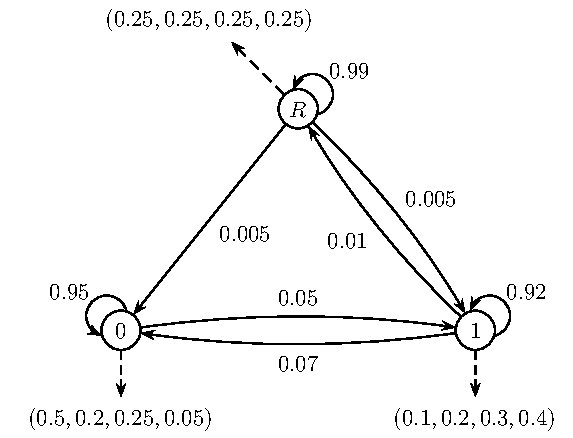
\includegraphics{../figures/exampleHMM.pdf}
\end{center}
\caption[Example of simple Hidden Markov Model]{
Example of HMM have $3$ states
that emits symbols from alphabet of size four.  Circles represents states, arc
from state $u$ to $v$ represents probability $a_{u,v}$. Missing arc from state
$In$ to $R$ means that $a_{In,R}=0$.  There are also arcs between states and
fourtouples. Everu fourtuple represents emmision distribution of it's state.
}\label{FIGURE:EXAMPLEHMM} 
\end{figure}


\begin{definition}\label{DEF:STATEPATH}
Let $H=(\Sigma,V,I,e,a)$ be an HMM. We say that there is \firstUseOf{transition}
form state $u$ to state $v$ if $a_{u,v}>0$. We will write transition from $u$ to
$v$ as $u\to v$ and $T=\{u\to v\mid a_{u,v}>0\}$ is set of all transitions of
$H$.

\firstUseOf{State path} $\pi=\pi_0\pi_1\dots\pi_{n-1}$ is a sequence of
states. We say that state path $\pi$ is \firstUseOf{admissible} if $I_{\pi_0}>0$
and  $\pi_{i-1}\to\pi_i\in T$ for all $1\leq i < n$. Otherwise $\pi$ is
\firstUseOf{inadmissible}.
\end{definition}

\begin{example}
Consider HMM from figure \ref{FIGURE:EXAMPLEHMM}. Set of transitions is
$T=\{R\to R,R\to In, R\to E,In\to In, In\to E, E\to E, E\to In, E\to R\}$.
State path $\pi_1=RRRRInER$ is admissible state path and $\pi_2=RRRInREER$ is inadmissible
state path, because contain transition with zero probability ($In\to R$).
\end{example}



%Formally, Hidden Markov Model is defined by it's finite state space
%$Q=\{q_0,q_2,\dots, q_{k-1}\}$ of size $k$, initial probabilistic distribution
%$I$ over state space, finite alphabet $\Sigma = (\sigma_0, \sigma_1, \dots,
%\sigma_{m-1})$ of
%size $m$, emission and transition distribution over $\Sigma$ and $Q$
%respectively defined for every state independently. We denote emission
%distribution of state $q$ by $e_q$ and transition distribution by $a_{q}$. 

Since Hidden Markov Models are generative probabilistic models, we have to
define probability distribution of HMM's products. In following definitions we
will define probability distribution of pairs (state path, sequence) and
probability distribution of sequences generated by HMM.

\begin{definition}
Let $H=(\Sigma,V,I,e,a)$ be an HMM and $X=X_0X_1\dots X_{n-1}$ be a sequence over
alphabet $\Sigma$ of length $n$. Let $\pi$ be a state path of length $n$. Then the
probability that state path $\pi$ generated sequence $X$ is 

\[\prob{X,\pi\mid H}=
I_{\pi_0}e_{\pi_0,X_0}\prod_{i=1}^{|X|-1}a_{\pi_{i-1},\pi_i}e_{\pi_i,X_i}\]

If length of the sequence $X$ is not equal to length of the state path $\pi$,
then
probability that $\pi$ generates $X$ is zero.
\end{definition}



\begin{example}
Consider HMM $H$ from example \ref{EXAMPLE:EXAMPLEHMM}. Let state path be $\pi=RRInInE$ and
generated sequence be $X=ACGTT$. Then the probability that $H$ generates $\pi$
and $X$ is 
$\prob{ X,\pi\mid H } = 0.5 \cdot 0.35 \cdot 0.99 \cdot 0.25 \cdot 0.005 \cdot 0.25 \cdot 0.95 \cdot 0.05 \cdot 0.05 \cdot 0.4 =
0.5143359375  \cdot  10^{-7}$
\end{example}

\begin{definition}
Let $H=(\Sigma,V,I,e,a)$ be a HMM and $X=X_0X_1\dots,X_{n-1}$ be sequence over
alphabet $\Sigma$ of length $n$. The probability that $X$ was generated by the
model $H$ is 
\[\Pr\left(X\mid H\right)=\sum_{\pi\in V^n}\Pr\left(X,\pi\mid H\right)\]
\end{definition}


%The probability of emission of sequence $X$ with state path $\pi$
%is \[\Pr\left(X,\pi\mid H\right) =
%I(\pi_0)e_{\pi_0}\left(X_0\right)\prod_{i=1}^{|X|-1}e_{\pi_i}a_{\pi_{i-1}}\left(\pi_i\right)\]
%Generally, there are many ways how to generate every sequence.  Therefore every
%HMM $H$ defines probability distribution \[\Pr\left(X\mid H\right) =
%\sum_{\pi,|\pi|=|X|}\Pr\left(X,\pi\mid H\right)\].  Since in every step HMM
%generates one symbol from $\Sigma$ and one state, state path has same length as
%generated sequence.

\begin{note}
In our  definition of an HMM, the sum of the probabilities of all sequences of
length $n$ is $1$. Later we will discuss concept of final states. With final
states, the sum of the probabilities of all sequences (of all lengths) is one.

%HMMs can have several final states.
%If final states are present, once HMM reach that state generation of a sequence
%stops. In this chapter we will ignore final states. \todo{Budeme ich vobec
%niekde potrebovat? Final states mozno a zdo poznamky za definiciouu
%pravdepodobnosti sevkvecie (ak ich
%bude treba)}
\end{note}

\todo{Tento text chcem dat asi trosku neskor, Az ked to budem potrebovat}
We will abuse the notation and by $e_q(\cdot)$ we mean row vector
$\left(e_{q,b_1},\dots,e_{q,b_{\sigma}}\right)$. Similarly,
$a_q(\cdot)=\left(a_{q,q_1},\dots,a_{q,q_k}\right)$ is row vector that contain
transition probabilities from the state $q$.  $a_q(\cdot)$ have therefore
dimension $1\times k$.
%By $A$ we will denote the $|Q|\times |Q|$ matrix
%consisting from vectors $a_{q_1},a_{q_2},\dots,a_{q_k}$.  Therefore $A[q_i,q_j]$
%contains probability of transition from state $q_i$ to $q_j$.

Usually there are three main problems associated with
HMMs\cite{}:
\begin{enumerate}
\item Given sequence $X$ and model $H$. What is the probability that $X$ was
generated by model $H$?
\item Given sequence $X$, model $H$ and assumption that $X$ was generated by 
$H$, what is the best explanation of $X$? By explanation is usually meant state
path that generated $X$. We call process of computing explanation from $X$ and
$H$ \firstUseOf{decoding}.
\item Given training data $D$ (usually sequences with ``explanations'') and
topology of model (set of states and transitions), what are the parameters
(initial, transition and emission distributions) that explains train
data?
\end{enumerate} 
In following sections we will discuss several algorithms
that are trying to solve problems describes above.



\section{Forward Algorithm}
The Forward algorithm \cite{Durbin1998} computes for a given sequence $X$ of
length $n$ the probability $\Pr\left(X\mid H\right)$ that sequence was
generated by the model (it solves first problem of HMM). The algorithm is based on dynamic programming. It fills
matrix $F$ of size $n\times m$ where $F[i,v]$ is the probability that $H$
generated $X[:i+1]$ with state path that ends in state $v$ and $m$ is the number
of states of $H$. Values $F[i,v]$ are also called \firstUseOf{forward
variables}. $F[i,v]$ can be computed by following formula.

\begin{align}
F[0,v] &= I_ve_{v,X_0}, v\in V\\
F[i,v] &= \sum_{u\in V}F[i-1,u] \cdot a_{u,v} \cdot e_{v,X_i}, v\in V,0< i < n
\end{align}
%We call values $F[i,v]$ forward variables. Value $F[i,v]$ is the
%probability, that $X[:i+1]$ was generated by state path that ends with state
%$v$. 
The probability that $H$ generated $X$ is 
 \[\Pr\left(X\mid H\right) = \sum_{v\in V} F[|X|-1,v]\]

Using the recurrence equations above, we can compute the probability of $X$ in
$O(nm^2)$ time and $O(m)$ memory dynamic programming where $n$ is the length
of the input sequence and $m$ is the number of states of $H$. If transition
matrix is sparse, then this algorithm can be implemented in $O(n(m+t))$ time
where $t$ is number of transitions.  Forward variables are also used in other
algorithms. 
%Storing all of the forward variables requires soring $O(nm)$ numbers.

\section{Sequence Annotation}

%definujeme annotation, footprint, set of colors

HMMs can be used for sequence annotation. By sequence annotation we mean
\todo{Predpokladam ze uz som v prvej kapitole vysvetlil co je gen a tak}
assigning ``labels'' to parts of the input sequence according to their meaning.
Now we give few examples.

\paragraph{Gene finding:} in living organisms parts of DNA sequences are
translated into proteins. Those parts of sequences which were used during
translation to proteins (we include also introns) are called genes. In gene
finding we want to find which parts of the input sequence are genes and which
are not. 

%For example in the gene-finding domain, we want to assign gene labels to those
%parts of the sequence that encode proteins. To annotate transmembrane proteins,
%we want to know, which parts of the sequence are on which  side of the membrane.
%In recombination prediction we want to predict which parts of the sequence
%belong to which subtype of an organism.  \todo{rozviest priklady, alebo zrusit}

\paragraph{Transmembrane proteins:} Some proteins in cells goes from one side of
membrane to other side of membrane (usually they pass membrane several times).
Aim of transmembrane proteins is to predict which parts of the protein sequence
is on which part of membrane and which parts are in membrane.

\paragraph{Recombination prediction:} Some organisms, for example HIV virus
, evolves rapidly and they have been classified into several subtypes.
Moreover, some viruses are mosaic combination of viruses from different
subtypes. For example beginning and end of RNA sequence of virus can be from 
one subtype and the middle of a sequence is from different subtype. In
recombination prediction we want to annotate RNA sequence of a virus by subtypes
from which that part of sequence originates.
\paragraph{}
In general, we have a finite set of labels $C=\{c_0,c_1,\dots,c_{l-1}\}$ and we
want to assign one label to every symbol of the input sequence. We do it by
assigning one label to every state of HMM.
%in a way, that states of HMM that
%encodes same meaning have same color. After that we try 
To predict the annotation of the input sequence $X$, we can for example find the
most probable state path that can generated $X$ and we annotate each symbol of
the sequence $X$ according to the label assigned to state that generated that
symbol. We can formalized this in the following way.

\todo{Aby nebol bordel medzi label a color}

\begin{definition}
Let $H=(\Sigma,V,I,e,a)$ be HMM and $C=\{c_0,c_1,\dots,c_{l-1}\}$ be the finite
sets of labels (or colors). Then \firstUseOf{coloring funcion} 
$\lambda: V^*\to C^*$ is function, that satisfies following properties:
\begin{enumerate}
\item $\lambda(v)\in C$ for all $v\in V$.
\item $\lambda(xy) = \lambda(x)\lambda(y)$ for all $x,y\in V^*$.
\end{enumerate}

Let $X$ be sequence generated by state path $\pi$. Then annotation
$\Lambda$ of sequence $X$ is $\Lambda = \lambda(\pi)$.
\end{definition}

In sequence annotation, we do not know the state path that generated a given
sequence. Our goal is to reconstruct the state path or at least to give a good
approximation of the correct annotation. Note that in general several state
paths can have the same annotation.

%Since many states of the HMM can have assigned same label, there may be may be
%many state path with same annotation.

\begin{definition}
Let $H$ be an $HMM$, $X$ be a sequence of length $n$, $\Lambda$ be an annotation of sequence
$X$. The probability of annotation $\Lambda$ given sequence $X$ is 
\begin{equation}
\Pr\left(\Lambda\mid X,H\right)=\sum_{\pi \in V^n,\lambda(\pi) =
\Lambda}\Pr\left(\pi\mid X,H \right)\label{DEF:ANNOTATION:PROBABILITY}
\end{equation}
\end{definition}

Note that $\prob{\pi\mid X,H}=\frac{\prob{\pi,X\mid H}}{\prob{X\mid
H}}$

\begin{example}\label{EXAMPLE:ANNOTATION}
Let $H$ be HMM from example \ref{EXAMPLE:EXAMPLEHMM}. Let $C=\{I,G\}$ and
$\lambda(R)=I$ and $\lambda(In)=\lambda(E)=G$.  Then annotation of sequence
$X=AACT$, which was generated by state path $\pi=RInEE$, is $\lambda(RInEE) =
IGGG$. 

We will use following interpretation of the model $H$. We can imagine $H$ as very simple gene
predictor\footnote{Not very realistic}. $R$ represents intergenic regions, state $In$
represents introns and $E$ represents exons. Annotation symbol $I$ represents
intergenic region and annotation symbol $G$ represents regions that are genes
(we recall that genes consists from introns and exons).

Using this interpretation, sequence $AACT$ contains gene $ACT$. There are
several explanations of this ``fact'': if $AACT$ was generated by state path
$REEE$ then subsequence $EEE$ is exone; if it was generated by state path $REIE$
then sequence contain two exons and one intron in the middle. There are $2^3$
different state paths $\pi$ with $\lambda(\pi)=IGGG$.  All of those state path
support ``fact'' that $IGGG$ is annotation of $X$.

\end{example}


%\begin{example}
%Consider again HMM from example \ref{EXAMPLE:EXAMPLEHMM} and annotation function
%from example \ref{EXAMPLE:ANNOTATION}.
%\end{example}

One natural question is, given sequence $X$ what is the best annotation of $X$.
One measure of quality of an annotation is it's probability. The more probable
is annotation, the more likely $X$ was generated with state path with such
annotation. We can formulate this in following problem.

\begin{definition}
Given HMM $H$ and sequence $X$, \abbreviation{the most probable annotation
problem}{MPA} is the problem of finding an annotation of $X$ that maximizes
the probability $\prob{\Lambda\mid X,H}$.
\end{definition}

\begin{theorem}
Most probable annotation problem is NP-hard.
\end{theorem}
This theorem was proved in 2002 by Lyngsø {\it et al.} and can be found in
\cite{Lyngso2002}. Their proof was done by conversion to maximal clique problem.
For input graph with $n$ vertices they construct HMM with $O(n^2)$ states and
sequence of length $n$ which most probable annotation could be converted into
maximal clique of input graph. 

\begin{theorem}
There exists an HMM such that it is HP-hard to find the most probable annotation
to given sequence $X$.
\end{theorem}
The proof of this theorem can be found in \cite{Brejova2007mpa}. This paper also
contain polynomial algorithm (Extended Viterbi Algorithm) that finds most
probable annotation for special classes of HMMs. 

\bigskip
{\large\bf Podtialto su zapracovane pripomienky}
\bigskip


\section{Viterbi Algorithm}
\todo{Viterbi variable ma rovnake oznacenie ako mnozina stavov. Treba to
upravit}
Viterbi algorithm is probably the most used decoding algorithm for Hidden Markov
models
Viterbi algorithm answer straightforward question: given the sequence
$X=X_0X_1\dots X_n$, what
is the most-likely state path $\pi$ that generates $X$? Formally, Viterbi
algorithm finds a state path maximizing $\Pr\left( \pi\mid X,H \right)$. Since
\[\Pr\left(\pi\mid X,H\right) = \frac{\Pr\left(\pi,X,\mid
H\right)}{\Pr\left(X\mid H\right)}\] and quantity $\Pr\left(X\mid H\right)$ is fixed
this is same as finding $\pi$ maximizing $\Pr\left(X,\pi\mid H\right)$. 

Viterbi algorithm is very similar to Forward algorithm. It starts with computing
Viterbi variables $V[i,v]$. $V[i,v]$ stores the probability of the most probable 
state path that generated $X[:i+1]$ and ends in state $v$. Viterbi algorithm
also computes back-links $B[i,v]$, which contains the previous state in the most
probable state path that generated $X[:i+1]$ and ends in state $v$. We can
compute these values by following equations:
\begin{align}
V[0,v] &= I_{v}e_{v,X_0}, v\in V\\
V[i,v] &= \max_{u\in V} V[i-1,u]a_{u,v}e_{v,X_i}, v\in V,0<i<n\\
B[i,v] &= \arg\max_{u\in V} V[i-1,u]a_{u,v}e_{v,X_i}, v\in V,0<i<n
\end{align}
\begin{note}
We do not specify how $B[0,v],v\in V$ is defined since we will not
need it to be defined in our computation.
\end{note}
\begin{note}
If we compare Viterbi algorithm with the Forward algorithm, we see that
Viterbi equations are forward equations if we replace summation with
maximization.
\end{note}

Variable $V[n-1,v]$ contains the probability of the most probable state path
that generated $X$ and end in state $v$. Therefore the state $v_{\max} =
\arg\max_{v\in V}V[n-1,v]$ is the last state of the most probable state path.
Variable $B[n-1,v_{\max}]$ contains the previous state of the most probable
state path. By traversing back through back-links  we can reconstruct the most
probable state path.

\begin{example}
Example of Viterbi Table with back-links
\end{example}

We can use Viterbi algorithm to annotate sequence $X$ by finding the most
probable state path $\pi$ and then computing $\lambda(\pi)$. In coloring
function $\lambda$ is identity function, this will find the most probable
annotation, but in general, Viterbi algorithm not even good approximation of the
most probable annotation.

\begin{example}
Why Viterbi is not good enough
\end{example}

\section{Backward Algorithm}
Backward algorithm is backward version of the Froward algorithm. ???
\section{Forward-Backward Algorithm and Posterior Decoding}
\firstUseOf{Posterior Decoding} is another commonly used decoding method. In
contrast to Viterbi algorithm, posterior decoding assign labels individually to
every symbol of input sequence and does not care about overall structure of
reconstructed state path. 

Given sequence $X$, posterior decoding find state path $\pi$ with following
property:
\[\forall 0\leq i< n, \pi_i=\arg\max_{v\in V}\Pr\left(\pi_i=v\mid X,H\right) \]
where \[\Pr\left(\pi_i=v\mid X,H\right) = \sum_{\pi\in V^n,\pi_i=v}\Pr\left(\pi\mid X,H\right)\]

Values $\Pr\left(\pi_i=v\mid X,H\right)$ can be computed with Forward-Backward
algorithm. This algorithm computes $\Pr\left(\pi_i=v\mid X,H\right)$ for every
combination of position $i$ and state $v$. Then for every position chooses state
that maximizes posterior probability.

Now we derive formula for effective computation of  $\Pr\left(\pi_i=v\mid
X,H\right)$.
\begin{align}
\Pr\left(\pi_i=v,X\mid H\right) &=  
%\sum_{\pi\in V^n,\pi_i=v}\Pr\left(\pi\mid X,H\right)
%					\label{PosteriorDer1} \\
%				&=& 
				\sum_{\pi\in
				V^n,\pi_i=v}I_{\pi_0}e_{\pi_0,X_0}\prod_{j=1}^{|X|-1}e_{\pi_j}a_{\pi_{j-1},\pi_j}
					\label{PosteriorDer2}\\
				&= \sum_{\pi\in V^n,\pi_i=v}I_{\pi_0}e_{\pi_0,X_0}
				\left( 
					\prod_{j=1}^{i-1} e_{\pi_j}a_{\pi_{j-1},\pi_j}
				\right)
				a_{\pi_{i-1},\pi_i}e_{\pi_i,X_i}
				\left(  
					\prod_{j=i+1}^{|X|-1} e_{\pi_j}a_{\pi_{j-1},\pi_j}
				\right)
					\label{PosteriorDer3}\\
				&= \sum_{\pi\in V^n,\pi_i=v}I_{\pi_0}e_{\pi_0,X_0}
				\left( 
					\prod_{j=1}^{i-1} e_{\pi_j}a_{\pi_{j-1},\pi_j}
				\right)
				a_{\pi_{i-1},v}e_{v,X_i}
				\left(  
					\prod_{j=i+1}^{|X|-1} e_{\pi_j}a_{\pi_{j-1},\pi_j}
				\right)
					\label{PosteriorDer4}\\
				&= 
				\left(
					\sum_{\pi\in V^{i+1},\pi_i=v}I_{\pi_0}e_{\pi_0,X_0}
					\left(
						\prod_{j=1}^{i} e_{\pi_j}a_{\pi_{j-1},\pi_j}
					\right)
				\right)
				\left( 
					\sum_{\pi\in V^{|X|-i},\pi_0=v}
					\prod_{j=1}^{|X|-i-1} e_{\pi_j}a_{\pi_{j-1},\pi_j}
				\right)
					\label{PosteriorDer5}\\
				&= F[i,v]
				\left( 
					\sum_{\pi\in V^{|X|-i},\pi_0=v}
					\prod_{j=1}^{|X|-i-1} e_{\pi_j}a_{\pi_{j-1},\pi_j}
				\right)
					\label{PosteriorDer6}
\end{align}
\todo{$e_{x}$ chyba jeden parameter.}
Equations \ref{PosteriorDer2} and \ref{PosteriorDer3} is from definition of
posterior probability. In \ref{PosteriorDer4} we just replace $\pi_i$ with $v$.
Next equality we have from the fact that the left part of the formula
\ref{PosteriorDer4} uses only left part of the state path and right part of the
formula uses only right part of the state path. Last equation follows from
definition of $F[i,v]$. Right part of the formula \ref{PosteriorDer6} has
similar structure than $F[i,v]$, but it uses last part of the state path and
sequence and also is lacks of using initial distribution. We can compute 
this formula using Backward algorithm, which is very similar to forward
algorithm. Let $B[i,v]$ be the right part of formula \ref{PosteriorDer6}.
\begin{align}
B[i,v]&=
\sum_{\pi\in V^{|X|-i},\pi_0=v}
	\prod_{j=1}^{|X|-i-1}
		e_{\pi_j,X_{|X|+j-1}}a_{\pi_{j-1},\pi_j}\\
 &= 
 \sum_{u\in V}
 	e_{u,X{|X|+j-1}}a_{v,u}
	\sum_{\pi\in V^{|X|-i},pi_0=v,\pi_1=u}
		\prod_{j=2}^{|X|-i-1}
			e_{\pi_j,X_{|X|+j-1}}a_{\pi_{j-1},\pi_j}\\
 &= 
 \sum_{u\in V}
 	e_{u,X{|X|+j-1}}a_{v,u}
	\sum_{\pi\in V^{|X|-i-1},pi_0=u}
		\prod_{j=1}^{|X|-i-2}
			e_{\pi_j,X_{|X|+j-2}}a_{\pi_{j-1},\pi_j}\\
 &= 
 \sum_{u\in V}
 	e_{\pi_j,X{|X|+j-1}}a_{\pi_0,\pi_1}B[i+1,u]
\end{align}
If we set $B[n,v]$ to $1$, we have recursive formula, to compute values
$B[i,v]$. This formula differs from Forward algorithm by going
backwards\footnote{Therefore it is called Backward algorithm.}.


Therefore \[\Pr\left(\pi_i=v\mid X,H\right) = \frac{F[i,v]\cdot
B[i,v]}{\Pr\left( X\mid H \right)}\]

We can compute this values in $O(nm^2)$ time and $O(nm)$ memory. By
check-pointing technique we can achieve $O(m^2\sqrt{n})$ memory requirements
with only constant slowdown.

As we can seem time complexity and memory requirement of posterior decoding is
same as for Viterbi algorithm, but in practice Forward-Backward algorithm is
slower and requires more memory.

Since posterior decoding does not care about overall structure of state path, it
can reconstruct inadmissible state path. One example is given below.
\begin{example}
Bad example
\end{example}

\section{Training} 

Training is process of estimating parameters of probabilistic models. In this
section we will describe several approaches how to estimate transition and
emission distributions. We will describe several approaches to do this thing

\subsection{Baum-Welsch algorithm}
\subsection{Viterbi Training}

Viterbi training is same as Baum-Welsch train

\subsection{Other Training Methods}
There are several other approaches how to similar
\section{Variants of Hidden Markov Models}

Hidden Markov models described in section \ref{SECTION:HMMDEF} are the Hidden
Markov models. In this section we describe several other variants of HMMs, some
of them with same expressing power and some not.

\subsection{Silent states}

One common variant of HMMs are HMMs with silent states. Silent state are states
that does not emit any symbol. One of the consequences is, that state path can
be longer then sequence. However, the number of non-silent states in state path
have to be equal to sequence length. Silent states does not add any expressing
power to HMMs, but in some cases they allow to reduce the number of transitions
by factor $m$.

\begin{definition}
Formally, Hidden Markov Model with silent states is tuple $H=(\Sigma,V,Q,I,e,a)$
where $\Sigma,V,I,a$ are defined as in definition \ref{DEF:HMM}. $Q\subseteq V$ is set of
silent states. $e$ must satisfy following conditions:
\begin{enumerate}
\item $\forall u\in V\backslash Q,\forall \sigma\in\Sigma, e_{u,\sigma}\geq0$
\item $\forall u\in Q,\forall \sigma\in\Sigma, e_{u,\sigma}=0$
\item $\forall u\in V\backslash Q, \sum_{\sigma\in \Sigma}e_{u,\sigma}=1$
\end{enumerate}
\end{definition}

\begin{definition}
Transitions and state path are defined as in definition \ref{DEF:STATEPATH}. 

Let $\pi$ be an state path. \firstUseOf{Non-silent state path} $\pi^Q$ is
maximal subsequence of $\pi$ that consists of non-silent states.
\end{definition}

\begin{definition}
Let $H=(\Sigma,V,Q,I,e,a)$ be a HMM and $X=X_0X_1\dots X_{n-1}$ be sequence over
alphabet $\Sigma$ of length $n$. Let $\pi$ be state path for which $\pi^Q$ have
length $n$. Then the probability that state path generated sequence $X$ is 

\[\Pr\left(X,\pi\mid H\right) =
I_{\pi_0}\left(\prod_{i=1}^{|\pi|-1}a_{\pi_{i-1},\pi_i}\right)\left(\prod_{i=0}^{|X|-1}e_{\pi^Q_i,X_i}\right)\]

If length of the sequence $X$ is not equal to length of the non-silent state
path $\pi^Q$, then
probability that $\pi$ generates $X$ is zero.
\end{definition}

\begin{example}
Example of HMM with silent states that reduces the number of edges by factor
$m$.

Consider following HMM: $H=(\Sigma,V,I,e,a)$ where
$|V|=m$, $I$ is arbitrary distribution over $V$, $e$ is also arbitrary and in
every row of $a$ is uniform distribution over $V$. In other words, there is
transition between any two pairs of states from $V$, that is exactly $n^2$
transitions\footnote{$u\to u$ is also transition}.

If remove all those transitions, add one silent state $s$ and add transitions
from state $s$ to all states from $V$ with probability $\frac1m$  and we add
transition from every state $V$ to $s$ with probability $1$. This new HMM
defines same distribution of sequences, but have one more state and only $2m$
transitions. 
\end{example}



\subsection{Start and Final state}

Sometimes it is useful to have special start state and special final state. We
will describe both states independently, since they affect models in different
ways. 

Having special start state $v$ is equivalent to $I_v=1$. 

HMM defined in section \ref{SECTION:HMMDEF} lacks conditions 
We can extend definition of HMMs to one or several final states.  


Final states affects distribution of model. HMM defined in section
\ref{SECTION:HMMDEF} define distribution over sequences of same length. HMM with
final states defines distribution over sequences of all length. 

\subsection{High Order HMMs}

If we look on the generated sequence as on the sequence of random variables
$X_0,X_1,\dots, X_{n-1}$ and if we look on the state path also as on the
sequence of random variables, $\pi_0,\pi_1\dots,\pi_{n-1}$, we observe that
$X_i$ depends only on $\pi_i$ and $\pi_i$ depends only on $\pi_{i-1}$ (Random
variables associated with state path have Markov property\cite{}). However,
sometimes ability to look back more then just one state/symbol is useful.

Therefore we can extend transition and emission probabilities to depend on
previous states/emissions. It is possible to depend on whole previous sequence,
however it increase running time of decoding and training algorithms by factor
of $n$. Therefore practical solutions that are using high-order HMM depends only
on small number of previous states/emissions.

\subsection{Generalized HMMs}

If we start observing then length of stay in one stay, we quickly end in 
with the conclusion that this is according geometric distribution.
The probability we will leave state $v$ after exactly $n$ steps is
$e_{v,v}^{n-1}(1-e_{v,v}$ which is geometric distribution. For some
applications in speech processing and ??? is this behaviour no appropriate.

\abbreviation{Generalized HMM}{GHMM} (or hidden semi-Markov model)
have with every state $v$ associated duration distribution $d_v(\cdot)$.  When
GHMM is in state $v$, it decides how long string it will generate according
$d_v$. Let it be $l$. Afterwards it generates string $x\in\Sigma^l$ with
probability $e_{v,x}$. Usually each symbol of generated string is generated
independently and then $e_{v,x}=\prod_{i=0}^{|x|-1}e_{v,x}$. Output of GHMM are
three sequences: state path $\pi=\pi_0\pi_1\dots\pi_{l-1}$, \firstUseOf{duration
sequence} $D=D_0D_1\dots D_{l-1}$ and sequence $X=X_0X_1\dots X_{n-1}$.  State
path and duration sequence has to have same length and \[\sum_{i=0}^{|D|-1}D_i =
|X|\].

Manipulation with GHMM is  more complicated and technical. If one state can
generate strings with various length then in general from state space we are
not able to uniquely assign to every state $v$ in $\pi$ the symbols from
sequence which were generated by $v$. To do so, we need also duration sequence.
Let $D^i = \sum_{i=0}^{i}D_i$ and $D^{-1}=0$.
The probability that $\pi$ with $D$ generated sequence $X$ is
\begin{equation}
\Pr(X,D,\pi\mid H) = 
\left(
\prod_{i=0}^{|\pi|-1}
d_{\pi_i}(D_i)e_{\pi_i,X[D^{i-1}:D_i]}
\right)
\prod_{i=1}^{|\pi|-1}
a_{\pi_{i-1},\pi_i}
\end{equation}
if $|\pi|=|D|$ and $|X|=\sum_{i=0}^{|D-1}D_i$. Otherwise $\Pr\left(X,D,\pi\mid
H\right)$ is zero. Similarly as with regular HMMs,  probability of the observed
sequence is
\begin{equation}
\Pr\left(X\mid H\right) = \sum_{\pi,D}\Pr\left(X,\pi,D\mid X\right)
\end{equation}
Computing this value can be done by variant of Forward algorithm. More details
in \cite{}. Maximizing likelihood of $\pi$ and $D$ can be found by variant of
Viterbi algorithm, also found in $\pi$.

%Generalized HMMs, or HMMs with explicit state duration density 

%Unlike hight order HMMs, emission and transition distribution depends only on
%current state. In \abbreviation{generalized hidden Markov model}{GHMM} every
%state can emit any finite string over alphabet $\Sigma$ according some
%distribution. This distribution can be, and usually is, different for every
%state. 

%Formally, each 
\section{Hidden Markov Models with Multiple Outputs}
In this section we will describe hidden Markov models that generates output on
two tapes -- they generates two sequences. These models are used in
bioinformatics to study relations between different sequences.

\subsection{Pair Hidden Markov Models}

Unlike previous variant of HMMs, \abbreviation{pair hidden Markov models}{pHMM}
are not equivalent to standard HMMs defined in section \ref{SECTION:HMMDEF}.
pHMM generates pair of sequences. Every state generate none or one symbol in
both sequences, one symbol in only one sequence or zero symbols in both
sequences. Formally, every state generates pair of strings $(a,b)$, where $|a|$
\todo{preformuluj zaver tohto odstavca} and $|b$ are of length at most one.
Moreover, once state generate some pair with nonzero probability, it can
generate only pairs with same length. Formal definition of pair HMM is given
below.

\begin{definition}
Pair hidden Markov model is tuple $H=(\Sigma,V,I,e,a)$, where $\Sigma$ is finite
alphabet, $V$ is final set of states and $I$ is initial distribution and $a$ is
transition matrix, all defined as
in definition \ref{DEF:HMM}. $e_{v,(\sigma_1,\sigma_2)}$ is
$|V|\times\left(|\Sigma|^2\right)$ matrix with following properties:
\begin{align} 
\forall v\in V\forall \sigma_1,\sigma_2\in\Sigma\cup\{\varepsilon\}:
e_{v,(\sigma_1,\sigma_2)}\geq 0\\
\forall v\in V:
\sum_{\sigma_1,\sigma_2\in\Sigma\cup\{\varepsilon\}}e_{v,(\sigma_1,\sigma_2)}\in
\{0,1\}\\
\forall v\in V\forall \sigma_1,\sigma_2\in\Sigma\cup\{\varepsilon\}: TODO
\label{DEF:PAIRHMM:UNIQ}
\end{align}
\todo{definition of $d^x$}
\end{definition}

State path is defined same as with HMMs. Equation \ref{DEF:PAIRHMM:UNIQ} ensures
\todo{Nepaci sa mi tato veta}
us that there is only one way ho to assign which symbols from sequences were
generated by which state. 

However, if we have only two sequences $X$ and $Y$ we are not able to tell which
symbols of the sequence were generated by same state. To do so, we have to had a
state path.
\begin{example}
Example of pair HMM (alignment?)
\end{example}

\begin{definition}
Let $H=(\Sigma,V,I,e,a)$ be an pair HMM, $X$ and $Y$ be arbitrary sequences over
$\Sigma$ and $\pi$ be state path. The probability that sequences $X$ and $Y$
were generated by model with state path $\pi$ is
\begin{equation}
\Pr\left(X,Y,\pi\mid H\right)=
I_{\pi_0}
\left(
	\prod_{i=1}^{|\pi|}a_{\pi_{i-1},\pi_i}
\right)
\left(
	\prod_{i=0}^{|\pi|}e_{\pi_i,(X[d^x_{i-1}:d^x_{i}],Y[d^y_{i-1}:d^y_{i}])}
\right)
\end{equation}
If $d^x_{|\pi|-1}\not=|X|$ or $d^y_{|\pi|-1}\not=|Y|$ then
$\Pr\left(X,Y,\pi\mid H\right)=0$ .
\end{definition}

\begin{definition}
Let $H=(\Sigma,V,I,e,a)$ be an pair HMM, $X$ and $Y$ be arbitrary sequences over
$\Sigma$. Then probability that sequences $X$ and $Y$ were generated together by
model is 
\begin{equation}
\Pr\left(X,Y\mid H\right)=\sum_{\pi}\Pr\left(X,Y,\pi\mid H\right)
\end{equation}
\end{definition}

\subsection{Viterbi algorithm for pair HMM}

Algorithm for manipulations with pHMM are similar to previous algorithm. Every
algorithm has it's pairwise version. In this section we will describe only two
dimensional version of Viterbi algorithm. Other algorithm are analogous.

Viterbi algorithm for HMM computes variables $V[i,v]$ and $B[i,v]$. Every
variable was parametrized by position in the sequence and state. For
two-dimensional version we will have to add position of the second sequence.

Let $V[i,j,v]$ be the probability of the most probable state path that generated
$X[:i+1]$ and $Y[:j+1]$ and ended in state $v$. Clearly, $\max_{v\in
V}V[|X|-1,|Y|-1,v]$ is the probability of the most probable state path that
generated $X$ and $Y$. Let $B[i,j,v]$ be the last but one state the most
probable state path that generated $X[:i+1]$ and $Y[:j+1]$ and ended in state
$v$.

Then
\begin{align}
V[i,j,v] &= \max_{u\in V}V[i-?,j-?,u]a_{u,v}e_{v,(?,?)}\\
V[-1,j,v] &= V[i,0,v] = 0 \\
V[0,0,v] &= I_{v}e_{v,(?,?)} \\
B[i,j,v] &= \arg\max_{u\in V}V[i-?,j-?,u]a_{u,v}e_{v,(?,?)}
\end{align}

Finding the last state $v$ of the most probable state path and back-tracing from
$B[|X|-1,|Y|-1,v]$ we can reconstruct the most probable state path. Time
complexity of this algorithm is $O(|X||Y||V|^2)$ and memory requirements are
$O(|X||Y||V|)$. However, we can use various tricks to decrease memory
requirements of such algorithms.

\subsection{Generalized Pair HMMs}


\abbreviation{Generalized pair HMM}{GpHMM} (or pair hidden semi-Markov
processes) are combination of $pHMM$ and $GHMM$.  Every state can emit like GHMM
generates two duration lengths $d^x$ and $d^y$ from some joint distribution
according current state $d_v(d^x,d^y)$ and after that it generates two strings
$x'$ and $y'$ with lengths $d^x$ and $d^y$ according joint distribution
$e_{v,(x',y')}$.  As with GHMM and unlike pHMM, just form the state path we are
not able tell which parts of the sequences were generated by which state. 

\begin{definition}
GpHMM is tuple $H=(\Sigma,V,I,e,a)$ where $\Sigma$ is finite alphabet, $V$ is 
\end{definition}

\section{Other Decoding Methods}
In the previous sections we described two decoding algorithm: Viterbi algorithm
that finds the most probable state path  and the Posterior decoding that
maximizes the expected number of correctly predicted states in state path.
\correction{We have shown}{Ak nie, umazat to} that in some cases these algorithm
recover bad annotation. However, maximizing the most probable annotation is
NP-hard and therefore it is not tractable.

In this section we will describe highest expected reward decoding framework and
some other decoding methods that were developed in recent years.

\subsection{Highest Expected Gain}

We will look on the decoding algorithm in more systematic way. We define gain
function, which will express similarity between
two annotations or state paths. The higher output, the more
similar those two sequences are. Gain function is not similarity in mathematical
sense and this function does not have to be even symmetric. 

Our goal is to find an annotation, that is as similar as possible to the correct
annotation. Problem is that we do not know the correct annotation. Our only
assumption is that data came from the model and therefore we will treat correct
annotation as the random variable, which is clearly defined by HMM and observed
sequence. We will seek for an annotation that maximizes the highest expected
gain.

\begin{definition}
Let $H$ be an HMM and $L$ be the set of all annotations. Any computable function
$f:L\times L\to \mathbb{R}$ is \firstUseOf{gain function}.
\end{definition}

\begin{note}
Gain functions are sometimes in literature called loss functions and lower loss
means more similar annotations. In such framework we want to minimize expected
loss. These two frameworks are equivalent.
\end{note}

\begin{definition}
Let $H$ be an HMM, $f$ be an gain function, $X$ sequence generated by $H$ and
$\Lambda$ annotation of $X$. Then \firstUseOf{expected gain} of annotation
$\Lambda$ is 
\begin{equation}
E_{\Lambda_X\mid X,H}[f(\Lambda_X,\Lambda)] =
\sum_{\Lambda_X}f(\Lambda_X,\Lambda)\Pr\left(\Lambda_X\mid X,H\right)
\end{equation}
\end{definition}


Once we have HMM $H$, gain function $f$ and observed sequence $X$,
we are trying annotation
\begin{equation}
\Lambda = \arg\max_{\Lambda}E_{\Lambda_X\mid
X,H}\left[f\left(\Lambda_x,\Lambda\right)\right]
\end{equation}

We can express previous decoding algorithm within this framework to show
its universality. We will define two gain functions $f_A, f_P$ one 
Viterbi algorithm and the most probable annotation problem and second for
posterior decoding.

\begin{equation}
f_A(\Lambda,\Lambda') = \begin{cases}
1 & \text{if $\Lambda = \Lambda'$ }\\
0 & \text{if $\Lambda \not=\Lambda'$}
\end{cases}
\end{equation}
If annotation function is identity function, then maximizing expected gain is 
equivalent to Viterbi algorithm since expected gain of annotation, which is
same as state path, is equal to it's probability.

In general, expected gain with function $g_A$ is equal to probability of such
annotation. Therefore finding annotation with highest expected gain is NP-hard
for arbitrary gain function.

\begin{equation}
f_P(\Lambda,\Lambda') = 
\begin{cases}
0 & \text{if $|\Lambda|\not=|\Lambda'|$}\\
\sum_{i=0}^{|\Lambda_1|}\begin{cases}
1 & \text{if $\Lambda_i=\Lambda'_i$}\\
0 & \text{otherwise}
\end{cases}
\end{cases}
\end{equation}

Again, if annotation function is identity, then finding annotation with maximal
expected gain $f_P$ is equivalent to Posterior decoding. 

Now we will show other decoding functions and their relations to

\subsection{Maximum Boundary Accuracy Decoding}

\abbreviation{Maximum boundary accuracy decoding}{MBAD}\cite{} is used in gene-finder
CONTRAST\cite{}. It
was proposed for \abbreviation{conditional random fields}{CRF}, but since CRF
are similar to HMM, we will defined them in the terms of HMM.

This decoding method tries to maximize weighted difference between the expected
number of true-positive and false-positive coding region boundaries.

\begin{definition}
Let $\Lambda=\Lambda_0\Lambda_1\dots\Lambda_{n-1}$ be an annotation. Boundary of
annotation $\Lambda$ is every position $i$ where $\Lambda_{i-1}\not=\Lambda_i$. 
\end{definition}

Maximum boundary accuracy decoding have one parameter $\kappa$. Let $B$ be the
set of all boundaries. Then MBAD maximize folowing function:
\begin{equation}
f(\Lambda,\Lambda')=\sum_{b\in B}
\begin{cases}
1 & \text{if $\Lambda_{i-1}=\Lambda'_{i-1}$ and $\Lambda_{i}=\Lambda'_{i}$}\\
-\frac1\kappa & \text{otherwise}
\end{cases}
\end{equation}

\subsection{Highest Expected Reward Decoding}

\abbreviation{Highest Expected Reward Decoding}{HERD} is extension of maximum
boundary accuracy decoding. We have used this decoding prediction of
recombination of HIV virus. In this subsection we will describe it's gain
function and basic properties. Further details can be found in \cite{} and in my
Master thesis\cite{}.


In the problem of recombination detection in virus RNA is usually jumping
HMM\cite{}. It is hard to find exact recombination point and annotations with
slightly shifted boundaries are very similar. Therefore we defined following
gain function.

Boundary on position $i$ is correctly predicted, if in the correct annotation is
same boundary (on position $j$) within distance $W$ symbols, if it is boundary
between same labels and if there is no other boundary between position $i$ and
$j$ in both annotations. Let $x$ be the number of correctly predicted boundaries
and $y$ be the number of other boundaries in the proposed annotation. Then
$f(\Lambda,\Lambda')=x-\gamma y$ where $\gamma$ is defined constant. If $W=1$
then this is equivalent to Maximum Boundary Accuracy Decoding.

Optimizing this criteria can be done in $O(nW|C||T| + n|C|^2W^2)$ time  and
$O(\sqrt{n}|C||V|+W|C||V|+n|C|^2)$ memory. Experimental evaluation of this
algorithm can be found in \cite{}.

\subsection{Distance Measures on Annotations}

Another approach to solve similar problem was proposed by {\it Brown,
Truszkowski} in \cite{}. Originally their implementation was aimed on prediction
of boundaries in transmebrane proteins\cite{}, but later they successfully
adapted their algorithm on jumping HMMs\cite{}.

\begin{definition}
Let $d$ be any distance measure defined on annotations. Ball of radius $r$
around annotation $\Lambda$ is 
\begin{equation}
B_d(\Lambda,r) = \{\Lambda'\mid d(\Lambda,\Lambda')\leq r\}
\end{equation}
\end{definition}

\begin{definition}
Let $\Lambda=\Lambda_0\Lambda_1\dots\Lambda_{n-1}$ be an annotations. Footprint
of $\Lambda$ is maximal subsequence of $\Lambda$ that does not contain two same
consecutive labels.
\end{definition}

{\it Brown,
Truszkowski} maximized following function
\begin{equation}
f_d(\Lambda,\Lambda') = 
\begin{cases}
\infty & \text{if $\Lambda$ and $\Lambda'$ have different footprint}\\
d(\Lambda,\Lambda') & \text{otherwise}
\end{cases}
\end{equation}

Where $d$ was either Hamming distance, Border shift distance or Border shift sum
distance\cite{}.


\subsection{Hybridizing Viterbi and Posterior Decoding}

There are approaches to combine Viterbi and Posterior decoding. It is
interesting that 


\section{Algorithmic improvements}
%balls, herd, hybridizing viterbi












